% geoweb.tex
\documentclass{beamer}
%\usetheme{roadkill}
%\usecolortheme[]{albatross}
\setbeamertemplate{navigation symbols}{} 
\usebackgroundtemplate{
	
\includegraphics[width=\paperwidth,
	height=\paperheight]{backdrop.png}
}
%\setbeamertemplate{itemize items}{\includegraphics[width=10px]{reflector.jpg}}

%\definecolor{safetyorange}{RGB}{232, 118, 0}
\setbeamercolor{background canvas}{bg=white}
\setbeamercolor{frametitle}{fg=black}
%\setbeamercolor{block title}{fg=white}
%\setbeamercolor{block body}{fg=white}
%\setbeamerfont{frametitle}{parent=structure,size=\huge}

\usepackage{graphicx}
\usepackage{datatool}
\usepackage{listings}
\usepackage{caption}
\usepackage{changepage}
\usepackage{amsmath}
\usepackage{amsfonts}
\usepackage{amssymb}
\usepackage{listings}

\usepackage{hyperref}
\hypersetup{colorlinks=true, linkcolor=blue, citecolor=blue, urlcolor=blue}


%Footnote like stuff
\usepackage[absolute,overlay]{textpos} 
\newenvironment{reference}[2]{% 
  \begin{textblock*}{\textwidth}(#1,#2) 
      \footnotesize\it\bgroup\color{black}}{\egroup\end{textblock*}} 

% items enclosed in square brackets are optional; explanation below
\title[PDFTitle]{Barriers to FOSS4G Adoption}
\subtitle[Sub]{OSGeo-Live case study}
\author[A. Mandel]{Alex Mandel, PhD} %\\
	%\footnotesize Co-Author: Paul Haverkamp}
\institute[UCD]{
  Geography Graduate Group\\
  University of California, Davis\\
  %Davis, California 95616\\[1ex]
  \texttt{aimandel@ucdavis.edu}\\
  @aimandel
}
\date[Sep 2014]{September 10, 2014}



\begin{document}
\section{Intro}
\begin{frame}[plain]
  \titlepage
   \begin{reference}{35mm}{85mm}
		\tiny \href{http://creativecommons.org/licenses/by-nc-sa/3.0/}{Creative Commons Attribution Share-alike Non-commercial}
		
\includegraphics[width=22px]{cc-a-nc-sa-88x31.png}
   \end{reference} 
  %\footnote{Creative Commons Attribution Share-alike Non-commercial}
\end{frame}

%\begin{frame}{Citizen Science aka Crowdsourcing}
%    \vspace{-1in}
%	\begin{itemize}
%		\item I
%			\begin{itemize}
%				\item A
%				\item B
%				\item C
%			\end{itemize}		
%		\item II
%			\begin{itemize}
%				\item A
%				\item B
%				\item C
%			\end{itemize} 
%	\end{itemize}
%\end{frame}

\begin{frame}{Definitions}
	\begin{itemize}
		\item Knowledge Diffusion - spread of awareness of an innovation
		\item Adoption - actual implementation of knowledge, innovation, or product
		\item Barrier - something that slows or stops the rate of diffusion or adoption \footnote{Barrier is a negative term, as opposed to studying how to increase rates.}
		\item Pro-innovation Bias - tendency to cast diffusion and adoption as positives
	\end{itemize}

\end{frame}



\begin{frame}{OSGeo-Live}
\begin{minipage}{\textwidth}
		\begin{center}
			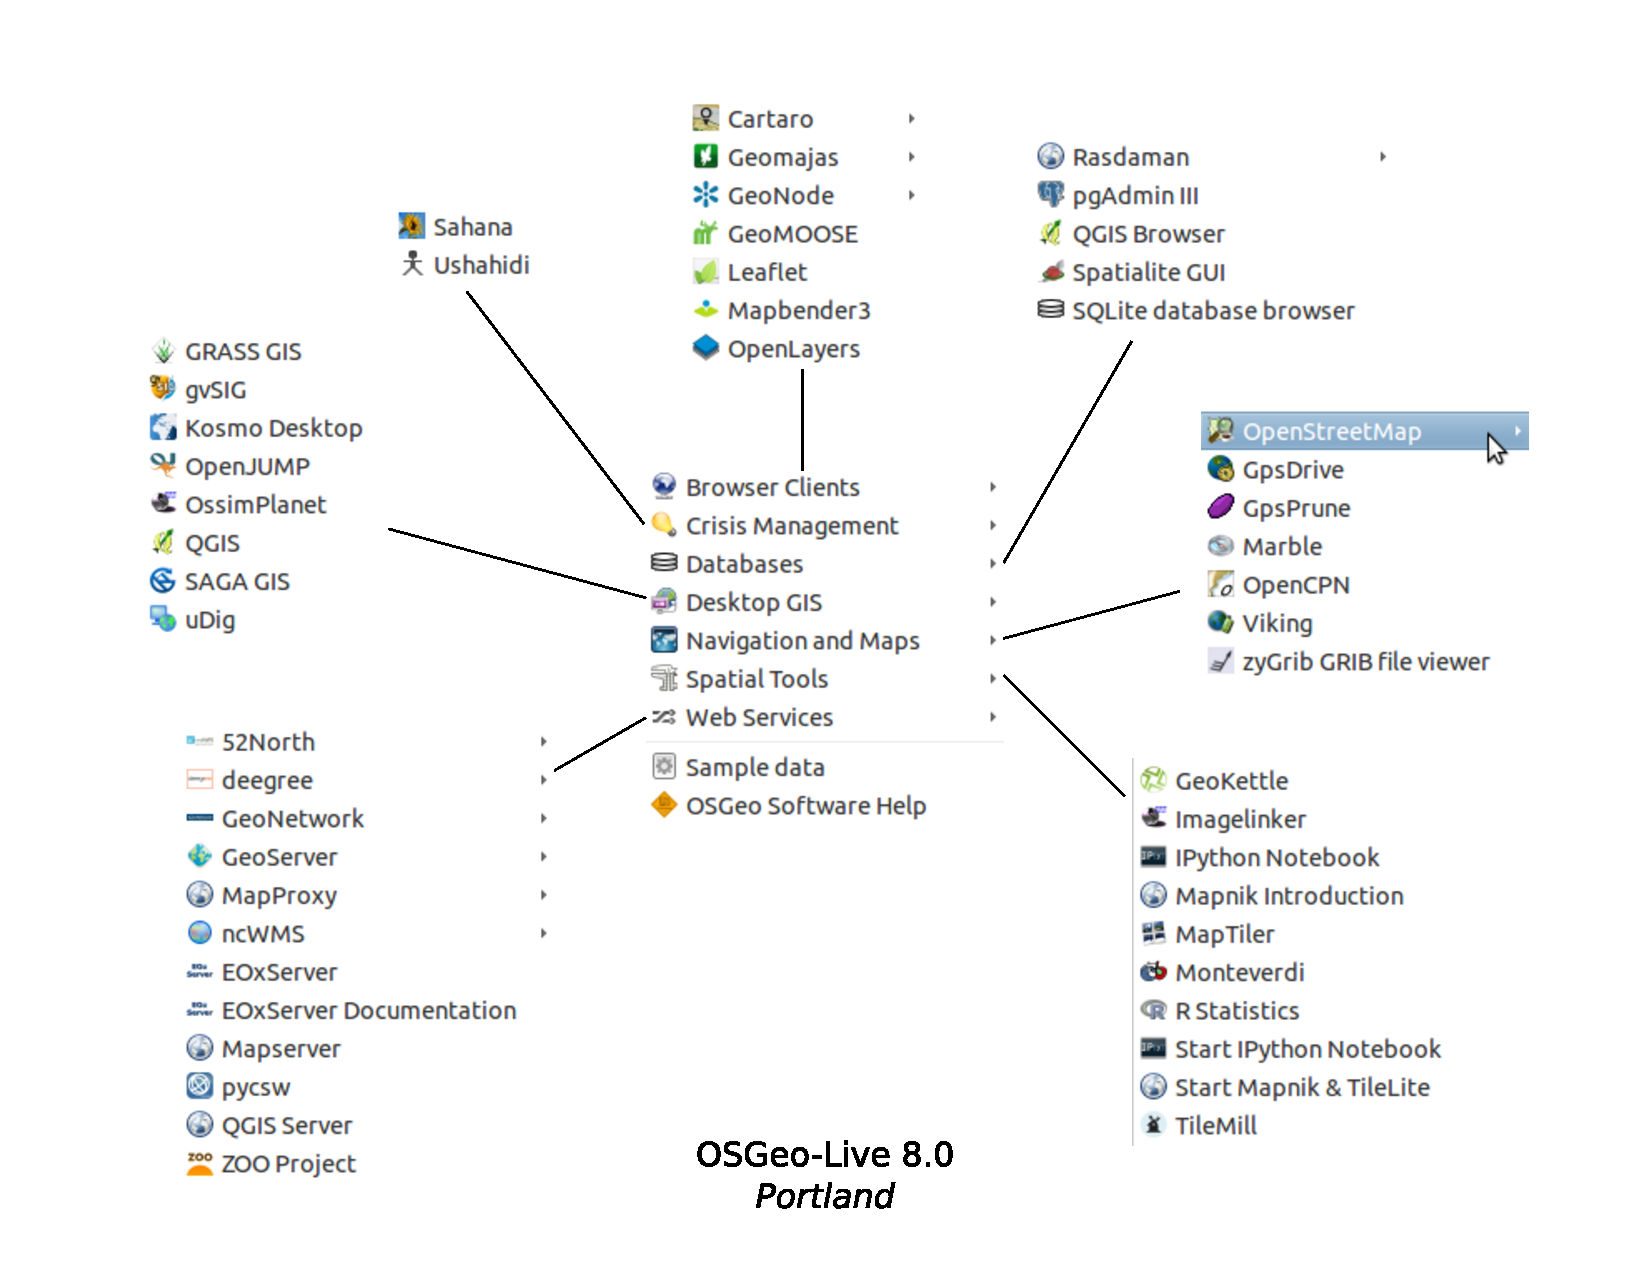
\includegraphics[width=1.0\textwidth]{livemenu8.pdf}
		\end{center}
		\url{http:://live.osgeo.org}
	\end{minipage}
\end{frame}

\section{Downloads}

\begin{frame}{History}
\vspace{-.25in}
	\begin{minipage}{\textwidth}
		\begin{center}
			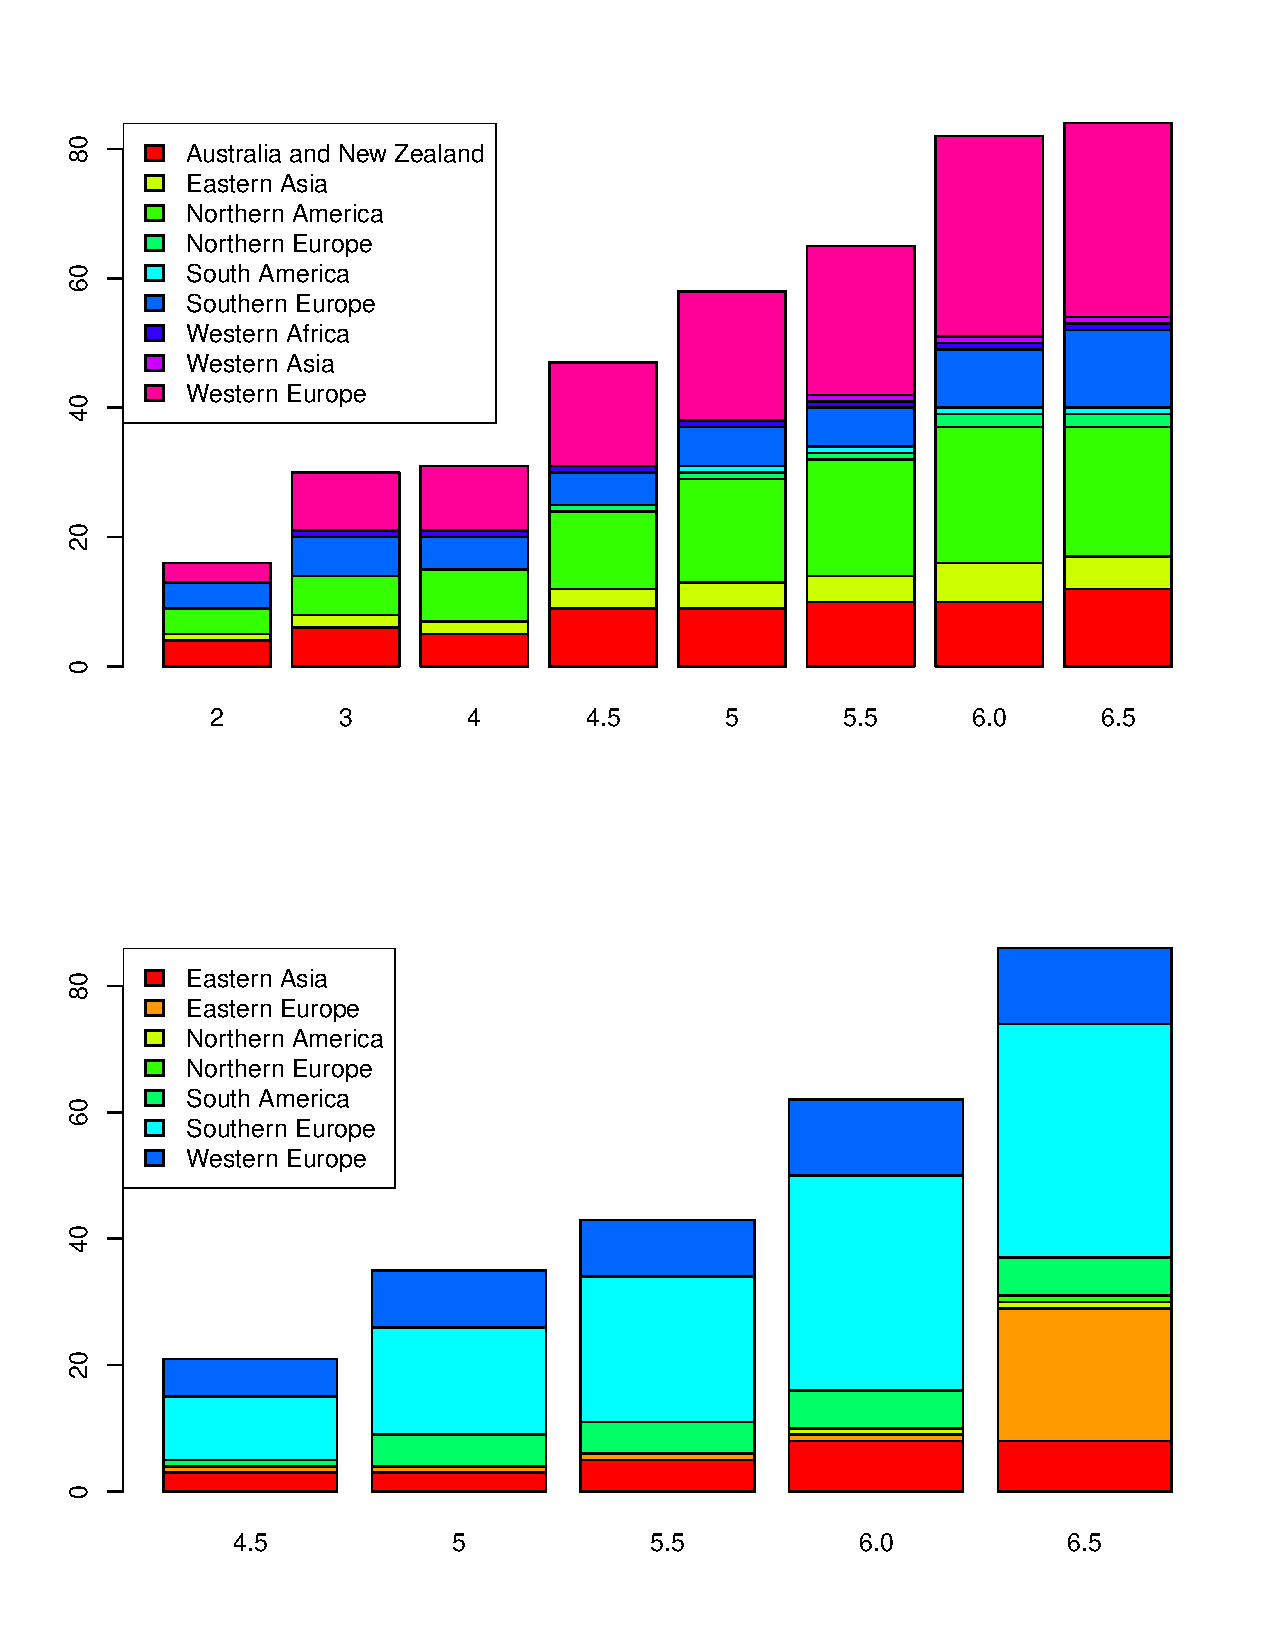
\includegraphics[width=0.6\textwidth]{OSGeoLiveInfographic.pdf}
		\end{center}
	\end{minipage}
%	\begin{reference}{35mm}{85mm}
%		\tiny {Projection: Van der Grinten I}
%  \end{reference} 
\end{frame}


\begin{frame}{Maps}
\vspace{-.25in}
	\begin{minipage}{\textwidth}
		\begin{center}
			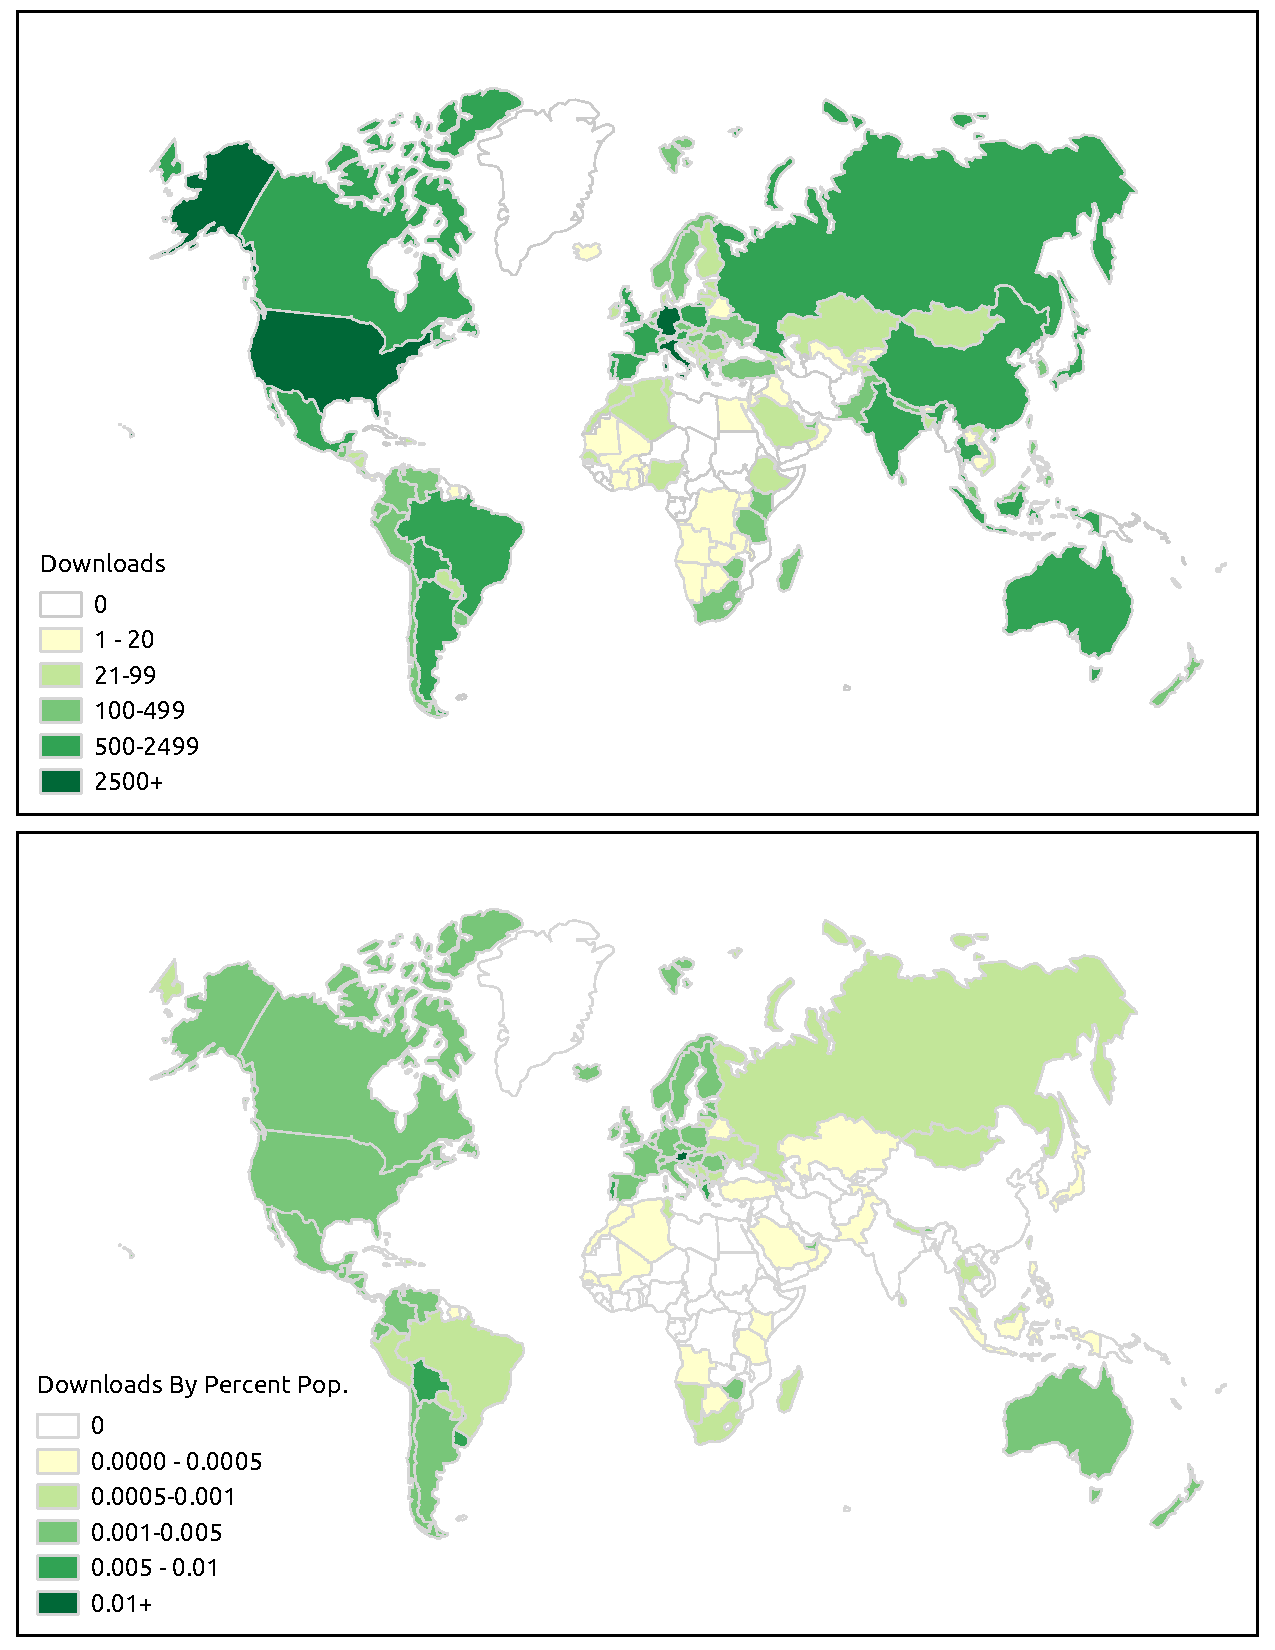
\includegraphics[width=.6\textwidth]{DownloadMapQGIS.pdf}
		\end{center}
	\end{minipage}
%	\begin{reference}{35mm}{85mm}
%		\tiny {Projection: Van der Grinten I}
%  \end{reference} 
\end{frame}

%All the date files
\DTLloadrawdb{top10down}{top10downloads.csv}
\DTLloadrawdb{top10downbypop}{top10downbypop.csv}
\DTLloadrawdb{top10linux-percent}{top10linux-percent.csv}
\DTLloadrawdb{top10linux-count}{top10linux-count.csv}
\DTLloadrawdb{top10mac-percent}{top10mac-percent.csv}
\DTLloadrawdb{top10mac-count}{top10mac-count.csv}

\begin{frame}{OSGeo-Live Downloads: Top 10 Countries \\ \tiny{(Versions 6.0 \& 6.5)}}
\vspace{-.5in}
	\begin{scriptsize}
	\begin{columns}[T]
	\begin{column}{0.3\textwidth}		
		\begin{table}
		\caption{\scriptsize{Total Downloads}}
		\begin{tabular}{l}
			\DTLdisplaydb{top10down}		
		\end{tabular}
		\end{table}
	\end{column}
	
	\begin{column}{0.001\textwidth}
	\end{column}
	
	\begin{column}{0.62\textwidth}
		
		\begin{table}
		%\centering
		\caption{\scriptsize{Downloads by Percent Population}}
			\begin{tabular}{l}
				\DTLdisplaydb{top10downbypop}
			\end{tabular}
		\label{table:top10}
		\end{table}
	\end{column}
	\end{columns}
	\end{scriptsize}
\end{frame}

\begin{frame}{Breakdown}
\vspace{-.3in}
	\begin{tiny}
	\begin{columns}[T]
	\begin{column}{0.5\textwidth}	
	
	\vspace{.2in}
	\centering
	{\normalsize Linux}
	\vspace{-.2in}
	
		\begin{table}
		\caption{\scriptsize{Total Downloads}}
		\begin{tabular}{l}
			\DTLdisplaydb{top10linux-count}		
		\end{tabular}
		\end{table}
		\vspace{-.3in}
		\begin{table}
		%\centering
		\caption{\scriptsize{Percent of Country's}}
			\begin{tabular}{l}
				\DTLdisplaydb{top10linux-percent}
			\end{tabular}
		\label{table:top10}
		\end{table}
	\end{column}
	
	\begin{column}{0.001\textwidth}
	\end{column}
	
	\begin{column}{0.5\textwidth}
		\vspace{.2in}
		\centering
		{\normalsize Mac}
		\vspace{-.2in}
		\begin{table}
		%\centering
		\caption{\scriptsize{Total Downloads}}
			\begin{tabular}{l}
				\DTLdisplaydb{top10mac-count}
			\end{tabular}
		\label{table:top10}
		\end{table}
		\vspace{-.3in}
		\begin{table}
		%\centering
		\caption{\scriptsize{Percent of Country's}}
			\begin{tabular}{l}
				\DTLdisplaydb{top10mac-percent}
			\end{tabular}
		\label{table:top10}
		\end{table}
		
	\end{column}
	\end{columns}
	\end{tiny}
\end{frame}


\begin{frame}{Significant Variation}
\centering
\begin{tiny}
\vspace{-.1in}
\begin{table}
\caption{\tiny World Internet connected desktop computers vs. OSGeo-Live downloaders.*}
\vspace{-.1in}
	\begin{tabular}{c | c c c c }
		%\hline
 		& Windows & Mac & Linux & Other \\ \hline
		Desktop Computers & 92.02000 & 6.810000 & 1.16000 & 0.000000 \\ 
		%OSGeo-Live Downloaders & 68.10947 & 6.738764 & 21.21359 & 3.938173 \\ 
		% From TotDownByOS View in db
		OSGeo-Live Downloaders & \textcolor{red}{68.6487} & 6.581052 & \textcolor{red}{20.78151} & 3.988733
	\end{tabular}
\end{table}
\vspace{-.2in}
\begin{table}
\caption{\tiny Operating System vs. OSGeo-Live variant downloaded.*}
\vspace{-.1in}
	\begin{tabular}{c | c c c }
		& vm & iso & mini	\\	\hline
		Windows& 8290 & 14822 & 5647 \\
		Mac& \textcolor{red}{1435} & 818 & 504 \\
		Linux& 2241 & 4031 & 2434 \\
		Other& 385 & 907 & 379 \\
	\end{tabular}
\end{table}

\end{tiny}
\vspace{-.3in}

\begin{center}
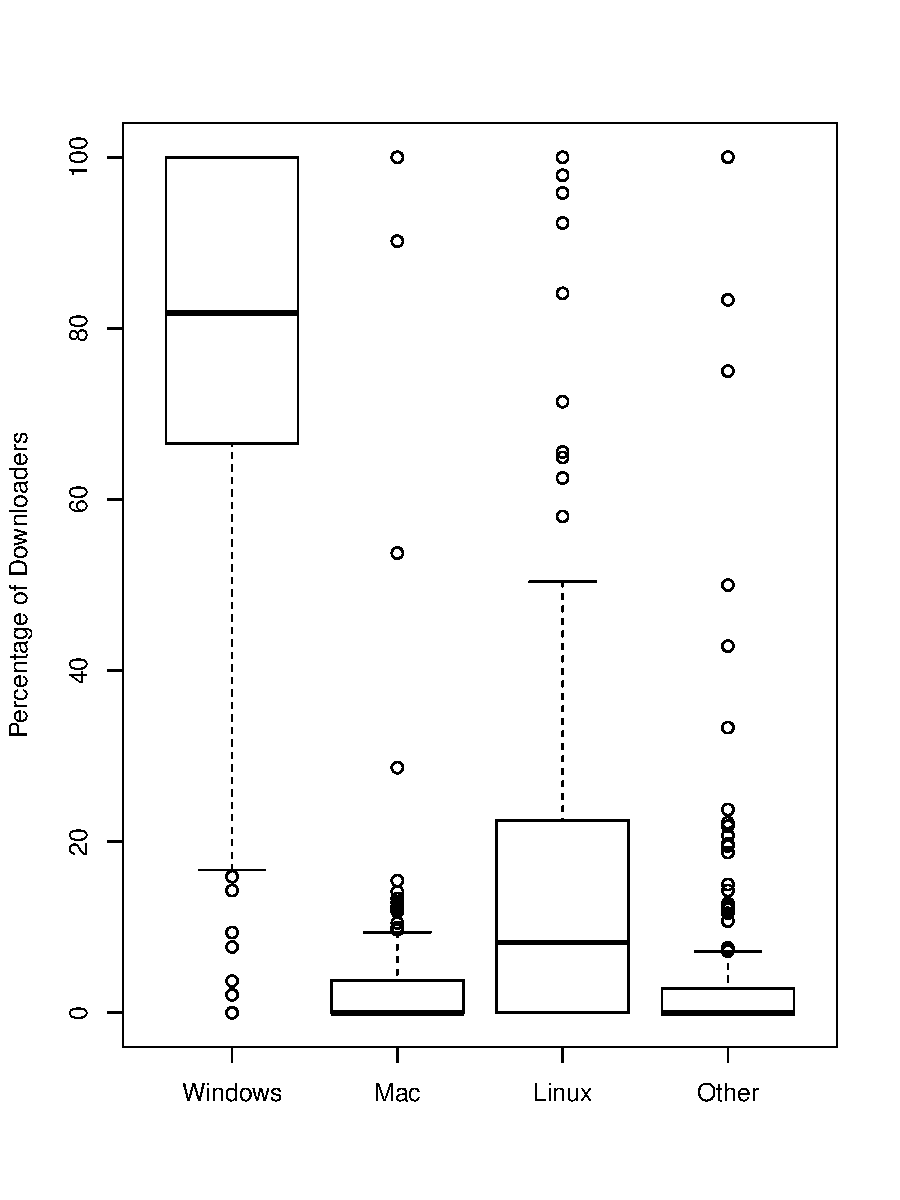
\includegraphics[width=.4\textwidth]{CountryOSVariation.pdf}
\end{center}
\vspace{-.1in}

\begin{reference}{11mm}{93mm}
\tiny{*Contingency table G-Statistic significant.}
\end{reference}

\end{frame}

\section{Participation}
\begin{frame}{Regional Participation}
\vspace{-.3in}
	\begin{center}
		%\hspace*{1em}
		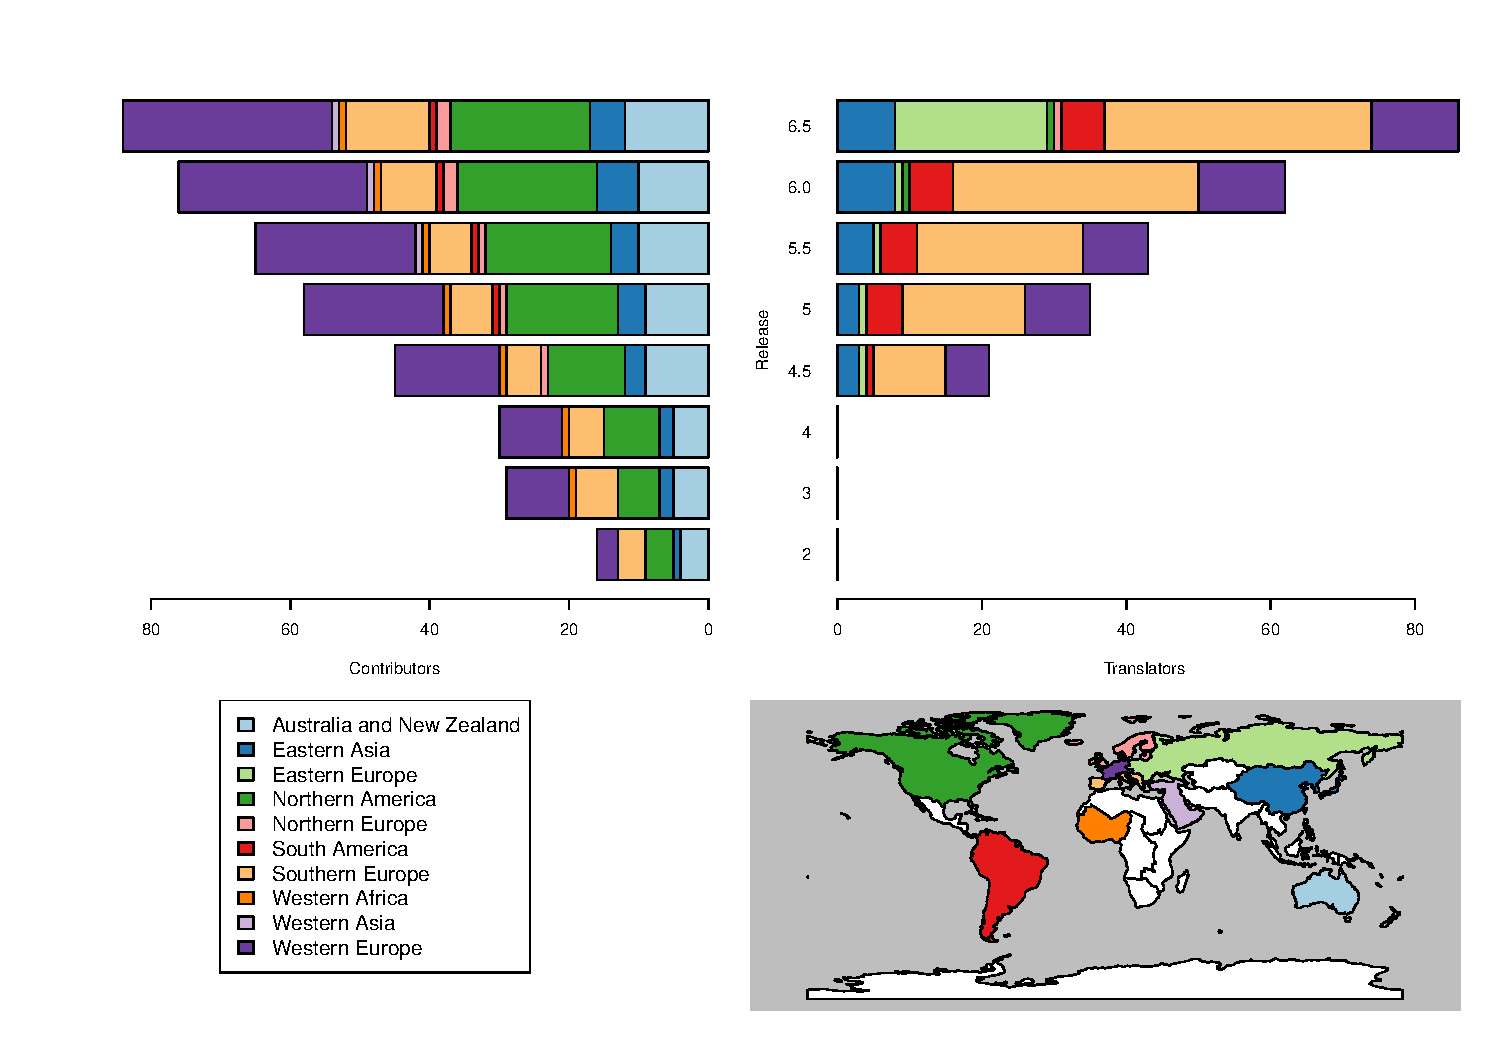
\includegraphics[width=1\textwidth]{RegionalParticipation.pdf}
		
		%\hspace*{2em}\textbf{\url{http://www.wildlifecrossing.net/california/}}
	
	Kendall's Rank Correlation, strong correlation, downloaders and participants $\tau = 0.436$ (p-value = 3.668e-12)	
	\end{center}
	
\end{frame}

\section{Analysis}

\begin{frame}{Barriers}
	\begin{itemize}
		\item Economic - License, Hardware, Education, Time
		\item Technical - Knowledge to operate software and hardware
		\item Socio-cultural - Government or Corporate Policy, Social Network 
	\end{itemize}
\end{frame}

\DTLloadrawdb{variables}{variables-horiz.csv}
\begin{frame}{Potential Barriers}
\vspace{-.3in}
	\begin{center}
		\begin{scriptsize}
			\DTLdisplaydb{variables}
		\end{scriptsize}
	\end{center}
\end{frame}

\begin{frame}[fragile]{Details}
\vspace{-.3in}
		%\centering
		\begin{scriptsize}
		\begin{columns}[T]
		\begin{column}{0.5\textwidth}
		%\subfloat[Economy Classification]{
			\begin{table}
			\caption{Economy Classification}
			\begin{tabular}{l}
				1. Developed region: G7\\ 
				2. Developed region: nonG7\\ 
				3. Emerging region: BRIC\\ 
				4. Emerging region: MIKT\\ 
				5. Emerging region: G20\\ 
				6. Developing region\\ 
				7. Least developed region\\		
			\end{tabular}
			\end{table}
		\end{column}
		%	\qquad
		%\subfloat[Income Classification]{
		\begin{column}{0.5\textwidth}
			\begin{table}
			\caption{Income Classification}
			\begin{tabular}{l}
					1. High income: OECD\\ 
					2. High income: nonOECD\\ 
					3. Upper middle income\\ 
					4. Lower middle income\\ 
					5. Low income
			\end{tabular}
			\end{table}
			%\label{table:econ-n-income}
		\end{column}
		\end{columns}
		
%		\begin{normalsize}
%			Regression Analysis with Random Forests
%		\end{normalsize}
		
		%\label{lst:cForest}
		\begin{lstlisting}[caption={Regression Analysis with Random Forests in R},label={lst:cForest},language={R},showspaces=false,breaklines=true]
#Packages: party, caret, to use multi-core: parallel, doMC 
mod1 <- train(downbypop ~ economy+income+OoklaAverage+ITUbroadband+AkUniqueIP+AkAverage+AkPeak+AkHighBroadband+AkBroadband+AkNarrowband+DemIndex, data = downdata,method = "cforest",trControl = trainControl(method = "oob",allowParallel = TRUE, number = 10, repeats = 10),controls = cforest_unbiased(ntree = 10000))
test.varimp <- varimp(mod1$finalModel,conditional=TRUE)		
		\end{lstlisting}
%		\begin{equation}
%			\begin{split}
%			\text{downbypop} \sim  &\text{ economy} + \text{income} + \text{OoklaAverage} + \text{ITUbroadband}\\
%			&+ \text{AkUniqueIP}+\text{AkAverage}+\text{AkPeak}+\text{AkHighBroadband}\\
%			&+ \text{AkBroadband}+\text{AkNarrowband}+\text{DemIndex}	
%			\end{split}
%			\label{eg:regression}
%		\end{equation}
		\end{scriptsize}
\end{frame}


\begin{frame}{Important Variables}
	\begin{center}
		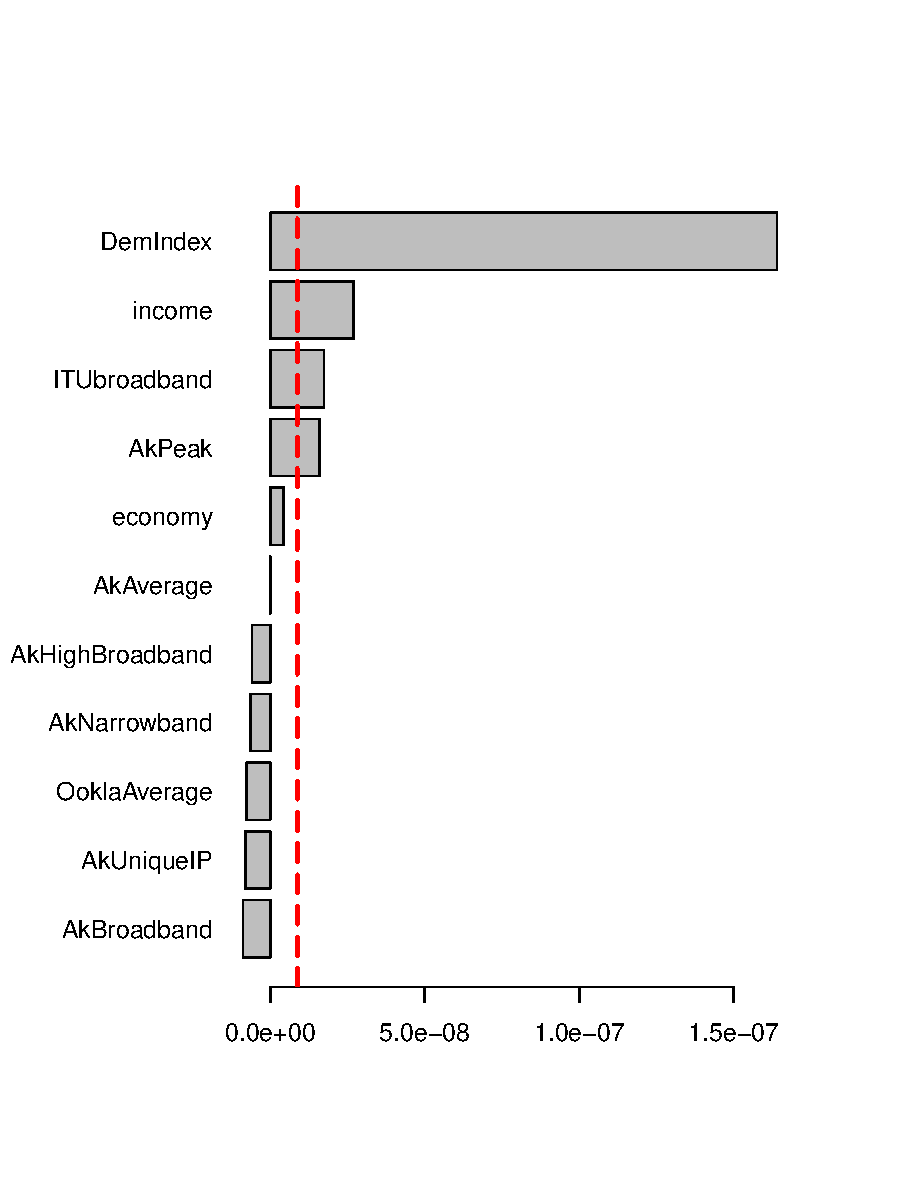
\includegraphics[width=.5\textwidth]{ImportantVariables-caret.pdf}
		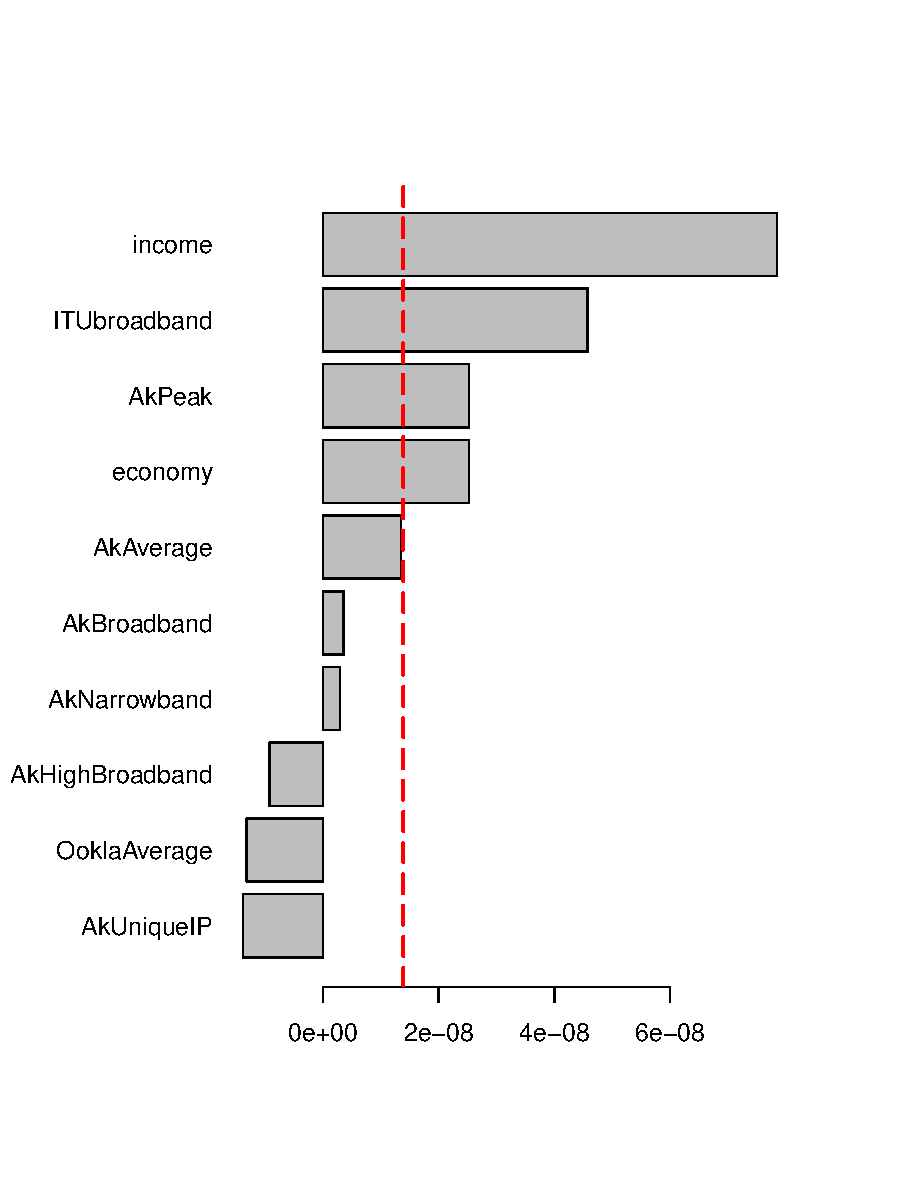
\includegraphics[width=.5\textwidth]{ImportantVariables-NoDemIndex.pdf}
	\end{center}
\end{frame}

\section{Regression}
\begin{frame}{Important Relationships}
	\begin{center}
			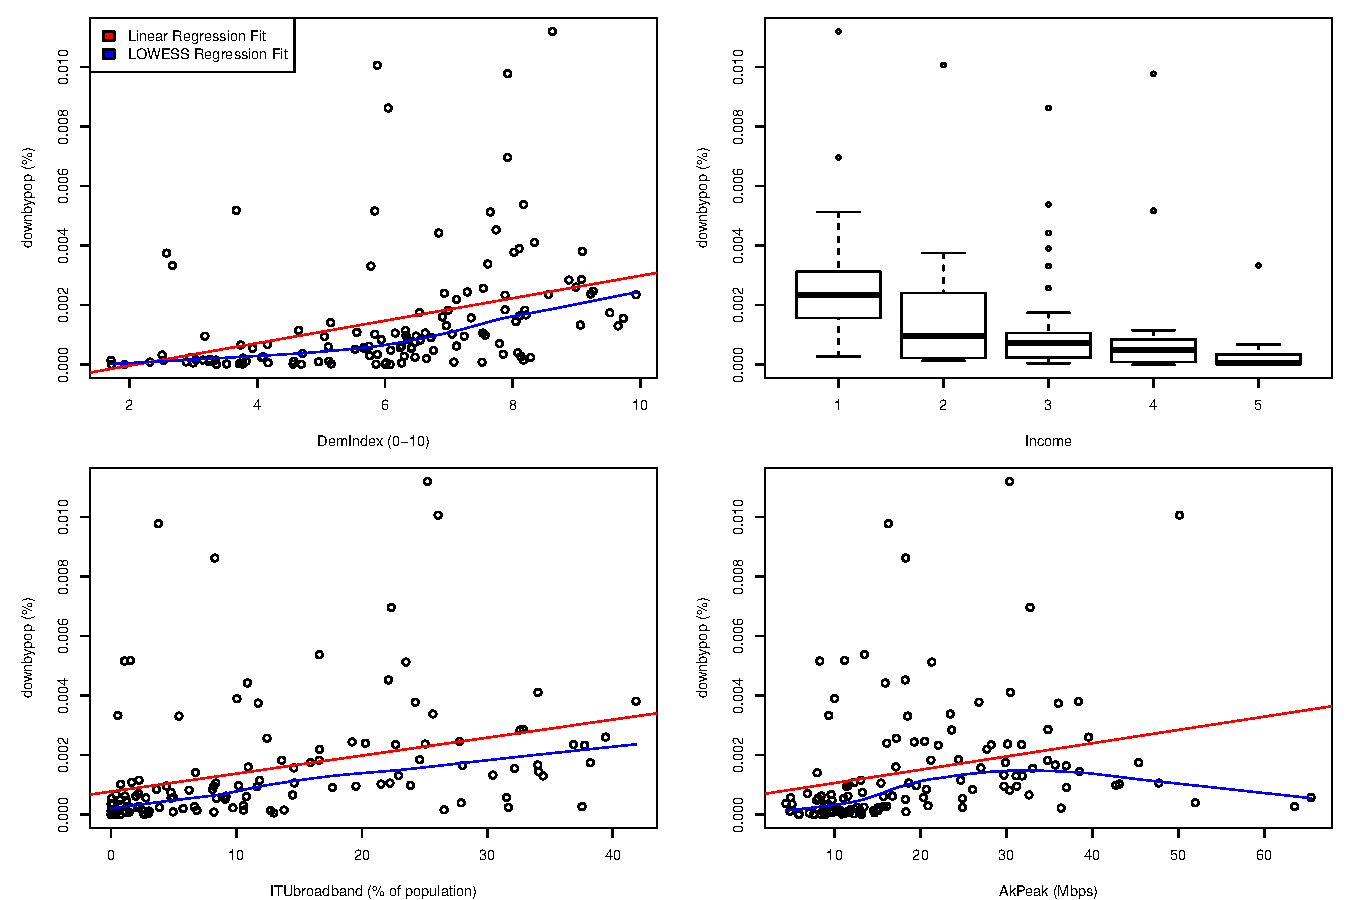
\includegraphics[width=1\textwidth]{ImportantVarGraph.pdf}	
	\end{center}
\end{frame}

\section{conclusion}
\begin{frame}{Conclusions}
	\begin{itemize}
		\item From the Data
		\begin{itemize}
			\item Mac users like Virtual Machines
			\item OSGeo-Live is popular with Linux users
			\item Having participants in the same country corresponds to downloads.
			\item Culture is a big barrier
			\item Fiscal and Technical issues still exist with FOSS
		\end{itemize}
		
		\item Key's to FOSS
		\begin{itemize}
			\item Infinite Trial-ability
			\item Re-invention potential
			\item Translation?
			\item Community
			\begin{itemize}
				\item Supply Side Institutions (e.g. OSGeo)
				\item Informal Social Networks (e.g. Local Chapters)
			\end{itemize}
		\end{itemize}				
		
	\end{itemize}
\end{frame}

\begin{frame}{What's Next}
	\begin{itemize}
			\item Confirmation \& Details - Survey Questionnaire
			\item How fast of internet is good enough?
			\item Compare Projects
			\item Test more specific data ...
			\begin{itemize}
				\item Household income
				\item English Proficiency
				\item \% of Higher Education
			\end{itemize}			 
			\item Change over time

	\end{itemize}
\end{frame}


\section{Credits}
\begin{frame}{Special Thanks}
	\begin{itemize}
		\item OSGeo-Live Team and Community \url{http://live.osgeo.org}
		\item Jim Quinn and the \href{http://ice.ucdavis.edu}{Information Center for the Environment}
		%\item Link Example %\begin{small}
%\url{http://www.wildlifecrossing.net/california/android}
%\end{small}
	\end{itemize}
			\begin{center}
			Questions?\\
			\url{http://github.com/wildintellect/?}\\
			@aimandel
			%\includegraphics[width=0.5\textwidth]{File.png}
		\end{center}
	

\end{frame}


% Columns example
%\begin{frame}{Currency of the GeoWeb}	
%		\begin{columns}[t]
%			\column{.59\textwidth} % column designated by a command
%     			\begin{block}{KML}
%      				%\tiny\lstinputlisting{world.kml}
%   				\end{block}
%    		\column{.39\textwidth}		
%				\begin{block}{GeoJson}
%					%\tiny\lstinputlisting{world.geojson}
%				\end{block}
%				\begin{itemize}
%					\item GML - not shown here
%				\end{itemize}
%		\end{columns}
%\end{frame}


\end{document}